
\chapter{Background}

This chapter present the fundamental concepts related to this work. The formal
definitions referring to fuzzy systems, user modeling concepts and gamification
theory and techniques related to this method.


\section{Fuzzy Logic.}

Fuzzy logic is an approach to computing based on "degrees of truth" rather than
the usual "true or false" (1 or 0) Boolean logic on which the modern computer is
based. The idea of fuzzy logic was first advanced by Dr. Lotfi Zadeh of the
University of California at Berkeley in the 1960s. Dr. Zadeh was working on the
problem of computer understanding of natural language. Natural language (like
most other activities in life and indeed the universe) is not easily translated
into the absolute terms of 0 and 1. (Whether everything is ultimately
describable in binary terms is a philosophical question worth pursuing, but in
practice much data we might want to feed a computer is in some state in between
and so, frequently, are the results of computing.) It may help to see fuzzy
logic as the way reasoning works, and binary or Boolean logic is simply a
special case of it. Fuzzy logic includes 0 and 1 as extreme cases of truth (or
"the state of matters" or "fact") but also includes the various states of truth
in between so that, for example, the result of a comparison between two things
could be not "tall" or "short" but ".38 of tallness."

Fuzzy logic seems closer to the way our brains work. We aggregate data and
create some partial truths which we aggregate further into higher truths which
in turn when certain thresholds are exceeded, cause certain further results such
as motor reaction. A similar kind of process is used in neural networks, expert
systems, and other artificial intelligence applications. Fuzzy logic is
essential to the development of human-like capabilities for AI, sometimes
referred to as artificial general intelligence: the representation of
generalized human cognitive abilities in software so that, faced with an
unfamiliar task, the AI system could find a solution.

\subsection{Fuzzy inference system.}

A fuzzy inference system (FIS) is a system that uses fuzzy set theory to map
inputs (features in the case of fuzzy classification) to outputs (classes in the
event of fuzzy classification). An example of a Mamdani inference system is
shown in Figure x To compute the output of this FIS given the inputs; one must
go through six steps:

\begin{enumerate}
\item \textbf{Determining a set of fuzzy rules.}
\item \textbf{fuzzifying the inputs using the input membership functions.}
\item \textbf{Combining the fuzzified inputs according to the fuzzy rules to establish a rule strength.}
\item \textbf{Combining the fuzzified inputs according to the fuzzy rules to establish a rule strength.}
\item \textbf{Combining the consequences to get an output distribution.}
\item \textbf{Defuzzifying the output distribution (this step is only if a crisp production (class) is needed).}
\end{enumerate}

The following is a more detailed description of this process.

\subsection{Creating fuzzy rules.}

Fuzzy rules are a collection of linguistic
statements that describe how the FIS should make a decision regarding
classifying an input or controlling an output. Fuzzy rules are always written in
the following form: if (input1 is membership function1) and/or (input2 is
membership function2) and/or . then (output is output membership function). For
example, one could make up a rule that says: if temperature is high and humidity
is high then room is hot. There would have to be membership functions that
define what we mean by high temperature (input1), high humidity (input2) and a
hot room (output1). This process of taking an input such as temperature and
processing it through a membership function to determine what we mean by "high"
temperature is called fuzzification and is discussed in section 3.1.2. Also, we
must define what we mean by "and" / "or" in the fuzzy rule. This is called fuzzy
combination and is discussed in section 3.1.3.

\subsection{Fuzzification.}

The purpose of fuzzification is to map the inputs from a set of sensors (or
features of those sensors such as amplitude or spectrum) to values from 0 to 1
using a set of input membership functions. In the example shown in figure \ref{fig:mamdaniFis},
there are two inputs, x0, and y0 is shown in the lower left corner.These inputs
are mapped into fuzzy numbers by drawing a line up from the inputs to the input
membership functions above and marking the intersection point.

\begin{figure*}
\captionsetup{justification=centering,margin=2cm}
\centering
\setlength\fboxsep{0pt}
\setlength\fboxrule{0.7pt}
\fbox{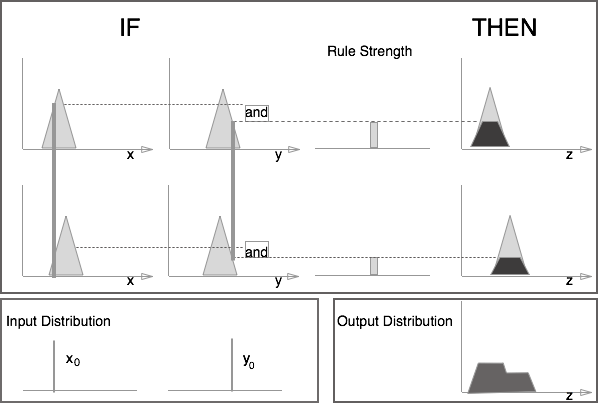
\includegraphics[width=10cm,height=10cm,keepaspectratio]{img/inference-sample.png}}
\caption{A two input, two rule Mamdani FIS with crisp inputs.}
\label{fig:mamdaniFis}
\end{figure*}

These input membership functions, as discussed previously, can represent fuzzy concepts
such as "large" or "small", "old" or "young", "hot" or "cold", etc. For example, x0
could be the EMG energy coming from the front of the forearm and y0 could be the
EMG energy coming from the back of the forearm. The membership functions could
then represent "large" amounts of tension coming from a muscle or "small"
amounts of tension. When choosing the input membership functions, the definition
of what we mean by "large" and "small" may be different for each input.

\subsection{Fuzzy combinations (T-norms).}
In making a fuzzy rule, we use the concept of "and", "or", and sometimes "not".
The sections below describe the most common definitions of these
"fuzzy combination" operators. Fuzzy combinations are also referred to as "T-norms".

\subsection{Fuzzy "and"}

The fuzzy "and" is written as:

\begin{equation}\label{eq:prediction}
\displaystyle \mu_A\cap \mu_B = T(\mu_A(x),\mu_ B(x))
\end{equation}

where µA is read as "the membership in class A" and µB is read as "the
membership in class B". There are many ways to compute "and". The two most
common are:

\begin{enumerate}
\item Zadeh - $min(\mu_A(x), \mu_B(x))$. This technique, named after the
inventor of fuzzy set theory simply computes the "and" by taking the minimum of
the two (or more) membership values. This is the most common definition of the
fuzzy "and".
\item Product - $\mu_A(x) + \mu_B(x)) - \mu_A(x) \mu_B(x))$. This technique uses the
difference between the sum of the two (or more) membership values and the
product of the membership values.
\end{enumerate}

Both techniques have the following properties:
\begin{itemize}
\item $T(a,0) = T(0,a) = a$
\item $T(a,1) = T(1,a) = 1$
\end{itemize}
Similar to the fuzzy "and", both
definitions of the fuzzy "or" also can be used to compute the Boolean "or".
Table \ref{tab:boolean_or} shows the Boolean "or" operation. Notice that both fuzzy "or" definitions
also work for these numbers. The fuzzy "or" is an extension of the Boolean "or"
to numbers that are not just 0 or 1, but between 0 and 1.

\begin{table}
\small
\caption{The Boolean "or".}
\label{tab:boolean_or}
\centering
\small
\begin{tabular}{p{3cm} p{3cm} p{3cm} }
\hline\noalign{\smallskip}
 Input 1 & Input 2 & Input 3 \\
\noalign{\smallskip}\hline\noalign{\smallskip}
\small{0} & \small{0} & \small{0}\\ \hline
\small{0} & \small{1} & \small{1}\\ \hline
\small{1} & \small{0} & \small{1}\\ \hline
\small{1} & \small{1} & \small{1}\\ \hline
\noalign{\smallskip}\hline
\end{tabular}
\end{table}

\subsection{Fuzzy "and"}

The consequence of a fuzzy rule is computed using two steps: 1. Computing the
rule strength by combining the fuzzified inputs using the fuzzy combination
process discussed in section 4.1.3. This is shown in Figure 4-1. Notice in this
example, the fuzzy "and" is used to combine the membership functions to compute
the rule strength. 2. Clipping the output membership function at the rule
strength. Once again, refer to Figure 4-1 to see how this is done for a two
input, two rule Mamdani FIS.

\subsection{Combining Outputs into an Output Distribution}
The outputs of all of
the fuzzy rules must now be combined to obtain one fuzzy output distribution.
This is usually, but not always, done by using the fuzzy "or". Figure 4-1 shows
an example of this. The output membership functions on the right-hand side of
the figure are combined using the fuzzy "or" to obtain the output distribution
shown in the lower right corner of the figure.

\subsection{Defuzzification of Output Distribution}

In many instances, it is desired to come up with a single crisp output from a
FIS. For example, if one was trying to classify a letter drawn by hand on a
drawing tablet, ultimately the FIS would have to come up with a crisp number to
tell the computer which letter was drawn. This crisp number is obtained in a
process known as defuzzification. There are two common techniques for
defuzzifying:

\begin{enumerate}
\item  Center of mass - This technique takes the output
distribution found in section 4.1.5 and finds its center of mass to come up with
one crisp number. This is computed as follows:
\begin{equation}\label{eq:centerM}
\displaystyle z=\frac{\sum_{j=1}^qz_j\mu_c(z_j)}{\sum_{j=1}^q\mu_c(z_j)}
\end{equation}

where z is the center of mass and uc is the membership in class c at value zj.
An example outcome of this computation is shown in Figure 4-2.


Falta agregar imagen al path
\begin{figure*}
\captionsetup{justification=centering,margin=2cm}
\centering
\setlength\fboxsep{0pt}
\setlength\fboxrule{0.7pt}
\fbox{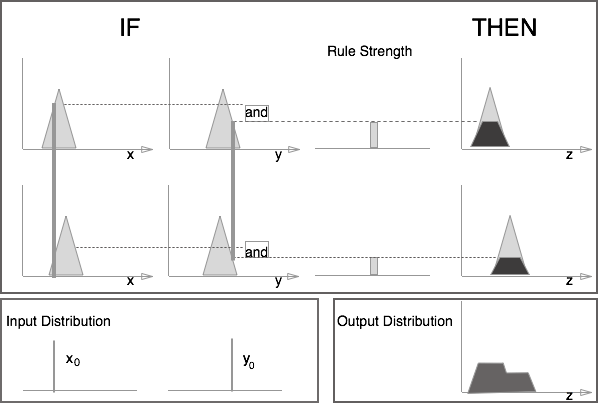
\includegraphics[width=10cm,height=10cm,keepaspectratio]{img/inference-sample.png}}
\caption{Defuzzification Using the Center of Mass.}
\label{fig:centerMass}
\end{figure*}



\item Mean of maximum - This technique takes the output distribution found in section
4.1.5 and finds its mean of maxima to come up with one crisp number. This is
computed as follows:
\begin{equation}\label{eq:centerM}
\displaystyle z=\frac{\sum_{j=1}^lz_j}{l}
\end{equation}

where z is the mean of maximum, zj is the point at which the membership function
is maximum, and l is the number of times the output distribution reaches the
maximum level. An example outcome of this computation is shown in Figure x.

Falta agregar imagen al path
\begin{figure*}
\captionsetup{justification=centering,margin=2cm}
\centering
\setlength\fboxsep{0pt}
\setlength\fboxrule{0.7pt}
\fbox{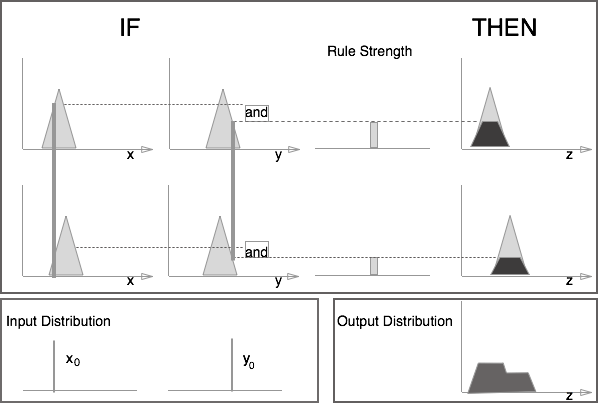
\includegraphics[width=10cm,height=10cm,keepaspectratio]{img/inference-sample.png}}
\caption{Defuzzification Using the Mean of Maximum.}
\label{fig:mean}
\end{figure*}

\end{enumerate}

\subsection{Fuzzy Inputs.}
In summary, Figure x-1 shows a two input Mamdani FIS
with two rules. It fuzzifies the two inputs by finding the intersection of the
crisp input value with the input membership function. It uses the minimum
operator to compute the fuzzy "and" for combining the two fuzzified inputs to
obtain a rule strength. It clips the output membership function at the rule
strength. Finally, it uses the maximum operator to compute the fuzzy "or" for
combining the outputs of the two rules. Figure x-4 shows a modification of the
Mamdani FIS where the input y0 is fuzzy, not crisp. This can be used to model
inaccuracies in the measurement. For example, we may be measuring the output of
a pressure sensor. Even with the exact same pressure applied, the sensor is
measured to have slightly different voltages. The fuzzy input membership
function models this uncertainty. The input fuzzy function is combined with the
rule input membership function by using the fuzzy "and" as shown in Figure x-4.

falta agregar el path de la imgen

\begin{figure*}
\captionsetup{justification=centering,margin=2cm}
\centering
\setlength\fboxsep{0pt}
\setlength\fboxrule{0.7pt}
\fbox{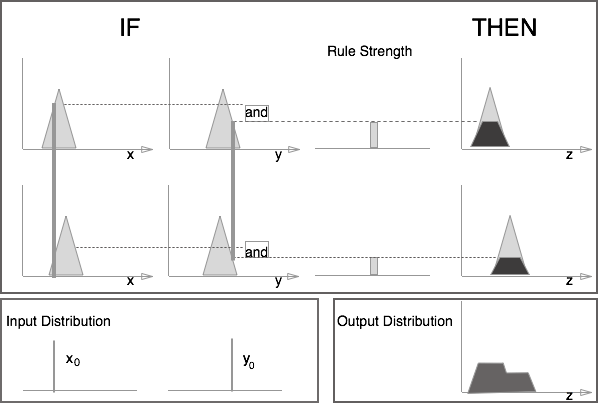
\includegraphics[width=10cm,height=10cm,keepaspectratio]{img/inference-sample.png}}
\caption{A two Input, two rule Mamdani FIS with a fuzzy output.}
\label{fig:fuzzyOut}
\end{figure*}
